\documentclass[border=0pt,10pt]{standalone}
\usepackage[T1]{fontenc}
\usepackage{lmodern}
\usepackage{pgfplots}
\pgfplotsset{compat=1.17}
\usepgfplotslibrary{groupplots}
\usepackage{xcolor}
\definecolor{oi-blue}{HTML}{0072B2}
\definecolor{oi-vermillion}{HTML}{D55E00}
\definecolor{oi-green}{HTML}{009E73}
\definecolor{oi-purple}{HTML}{CC79A7}
\definecolor{oi-black}{HTML}{000000}
% semantic_sha256: bd2a953e6fdeba82f892112e77e569b479863bd0d1672a21f119ca1f80c333bc
\begin{document}
\begin{minipage}{181.86mm}
\centering
{\bfseries\fontsize{10}{12}\selectfont PP-U-SG | D1 | source\_fit}\\[2mm]
{\fontsize{8}{10}\selectfont planned=108, monitored=105, missing-history=3, status=partial\_history\_coverage}\\[3mm]
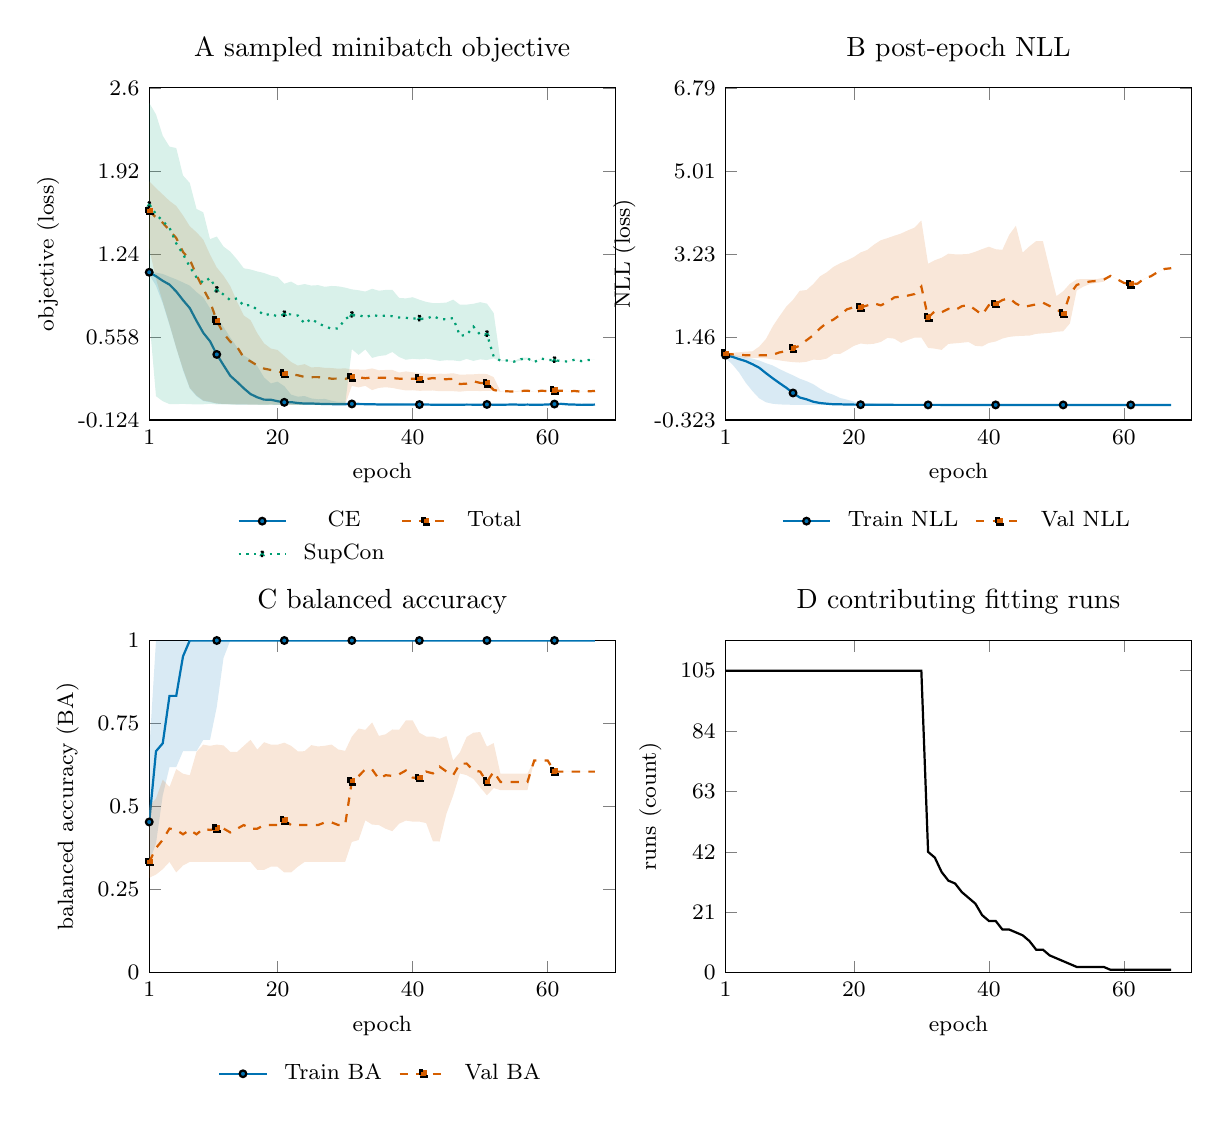
\begin{tikzpicture}
\begin{groupplot}[group style={group size=2 by 2, horizontal sep=14mm, vertical sep=28mm}]
\nextgroupplot[width=75mm, height=58mm, title={A sampled minibatch objective}, xlabel={epoch}, ylabel={objective (loss)}, xmin=1, xmax=70, xtick={1,20,40,60}, ymin=-0.12394953787326812, ymax=2.6029402953386307, ytick={-0.12394953787326812,0.55777292042970661,1.2394953787326815,1.9212178370356559,2.6029402953386307}, yticklabels={-0.124,0.558,1.24,1.92,2.6}, tick label style={font=\fontsize{8}{9}\selectfont, text=black}, label style={font=\fontsize{8}{9}\selectfont, text=black}, title style={font=\fontsize{10}{11}\selectfont, text=black}, legend style={at={(0.5,-0.24)},anchor=north,draw=none,fill=none,font=\fontsize{8}{9}\selectfont,row sep=1pt,column sep=4pt,legend columns=2}]
\addplot[fill=oi-blue,opacity=0.15,draw=none,forget plot] coordinates {(1,1.0708940267562865) (2,0.97870230674743652) (3,0.83521417677402499) (4,0.65615304708480837) (5,0.46784728765487671) (6,0.28590905517339704) (7,0.13584827333688737) (8,0.072271225042641163) (9,0.032444186974316835) (10,0.022556854179129004) (11,0.010715514281764628) (12,0.0064094264875166123) (13,0.0053337247751187537) (14,0.0031520077667664737) (15,0.003210433793719858) (16,0.0020831004425417633) (17,0.0015566068555926908) (18,0.0016992387594655157) (19,0.0017434604611480608) (20,0.0012148619920480997) (21,0.0010680819083063397) (22,0.00098134253057651226) (23,0.00067642586509464309) (24,0.0010405606968561187) (25,0.0011361628385202494) (26,0.00081487612987984903) (27,0.0007757536674034782) (28,0.00041387452147318983) (29,0.00063459613884333523) (30,0.0007585413637571037) (31,0.0024924389548687032) (32,0.0022105828189523894) (33,0.0018507312226574873) (34,0.0017840519707533532) (35,0.00093931344599695876) (36,0.0022109987563453614) (37,0.0012452139162633102) (38,0.0010271276545608999) (39,0.0014150398361380213) (40,0.0014541568936692786) (41,0.00086037869441497623) (42,0.00051784406350634531) (43,0.0012627856252947823) (44,0.00091922710016660862) (45,0.00051450345636112622) (46,0.00050111248674511444) (47,0.00045166864656494006) (48,0.0012274863365746569) (49,0.0010156592561543221) (50,0.00156305565033108) (51,0.0033030828752089294) (52,0.001452265607076697) (53,0.0011829743802081794) (54,0.001975847397989128) (55,0.0029495131908333859) (56,0.0010212932116701267) (57,0.0027310880162985996) (58,0.0012495633854996413) (59,0.0018274740286869928) (60,0.0037085244548507035) (61,0.0072993973881239071) (62,0.0090109658776782453) (63,0.0045015385512670036) (64,0.0028369250649120659) (65,0.00060736158775398508) (66,0.0010203530546277761) (67,0.0028603755745280068) (67,0.0028603755745280068) (66,0.0010203530546277761) (65,0.00060736158775398508) (64,0.0028369250649120659) (63,0.0045015385512670036) (62,0.0090109658776782453) (61,0.0072993973881239071) (60,0.0037085244548507035) (59,0.0018274740286869928) (58,0.0012495633854996413) (57,0.0028485468152211978) (56,0.0022650426821201109) (55,0.0040288883596076627) (54,0.003006976122560445) (53,0.0026132519065868109) (52,0.0036077431548619645) (51,0.0052347745717270305) (50,0.0058955362706910822) (49,0.0069365372328320518) (48,0.0034280852843949104) (47,0.0015400469230371528) (46,0.0050915561296278611) (45,0.0037713742931373417) (44,0.0050194405805086733) (43,0.0041995495324954387) (42,0.0082434233976528028) (41,0.005218597366729227) (40,0.0068765988027735155) (39,0.0090477698919130493) (38,0.011415075755212454) (37,0.01351022205199115) (36,0.013174638661439532) (35,0.012502208235673606) (34,0.015584915730869398) (33,0.015318700588250068) (32,0.020679307240061465) (31,0.017480043234536422) (30,0.028447155782487299) (29,0.024717751075513671) (28,0.03440839136019351) (27,0.049549528677016598) (26,0.046389736304991061) (25,0.053342717699706568) (24,0.073127192072570374) (23,0.067916229274123996) (22,0.084743203595280717) (21,0.15412043854594254) (20,0.19133648276329052) (19,0.17646403759717946) (18,0.22598904445767409) (17,0.31868846267461792) (16,0.37401716560125353) (15,0.40593947172164918) (14,0.47302310764789585) (13,0.5539994657039643) (12,0.63969005346298224) (11,0.72340380251407621) (10,0.79318254590034487) (9,0.88176417946815489) (8,0.92642898261547091) (7,0.97893774509429932) (6,1.0056109100580215) (5,1.0305738329887391) (4,1.0521457374095917) (3,1.0752083957195282) (2,1.0858788549900056) (1,1.1038019835948945)};
\addplot[color=oi-blue, mark=*, mark options={draw=black}, mark repeat=10, mark size=1.2pt, solid, line width=0.8pt] coordinates {(1,1.0891026556491852) (2,1.0567274987697601) (3,1.0191532075405121) (4,0.98780715465545654) (5,0.93147894740104675) (6,0.86016032099723816) (7,0.79526656866073608) (8,0.68985852599143982) (9,0.59224028885364532) (10,0.52287557721138) (11,0.41465172171592712) (12,0.32635249197483063) (13,0.23930482566356659) (14,0.18952322006225586) (15,0.13652214780449867) (16,0.089309243485331535) (17,0.06264499481767416) (18,0.043608196079730988) (19,0.042844903655350208) (20,0.030682560056447983) (21,0.021442511584609747) (22,0.022866635001264513) (23,0.015886156819760799) (24,0.011339858407154679) (25,0.012181042693555355) (26,0.0091883238055743277) (27,0.00771881896071136) (28,0.0065919357584789395) (29,0.0055472024250775576) (30,0.0060871458263136446) (31,0.0082503353551146574) (32,0.0068648813758045435) (33,0.006424863007850945) (34,0.0056698356638662517) (35,0.0037475405988516286) (36,0.0044680858554784209) (37,0.0038261880981735885) (38,0.0037684395501855761) (39,0.0036726753460243344) (40,0.0044295580592006445) (41,0.0031460373793379404) (42,0.0032689677900634706) (43,0.001931887396494858) (44,0.0019550341876310995) (45,0.0022916618472663686) (46,0.0021320703672245145) (47,0.0012040028450428508) (48,0.0027481679280754179) (49,0.0022932026549824513) (50,0.0019921472412534058) (51,0.004018218707642518) (52,0.0018108723015757278) (53,0.0018981131433974952) (54,0.0024914117602747865) (55,0.0034892007752205245) (56,0.0016431679468951188) (57,0.0027898174157598987) (58,0.0012495633854996413) (59,0.0018274740286869928) (60,0.0037085244548507035) (61,0.0072993973881239071) (62,0.0090109658776782453) (63,0.0045015385512670036) (64,0.0028369250649120659) (65,0.00060736158775398508) (66,0.0010203530546277761) (67,0.0028603755745280068)};
\addlegendentry{CE}
\addplot[fill=oi-vermillion,opacity=0.15,draw=none,forget plot] coordinates {(1,1.2845683574676514) (2,1.0359338492155075) (3,0.84693730175495152) (4,0.66445039212703705) (5,0.46950371712446215) (6,0.29556918889284134) (7,0.14125883206725121) (8,0.077827091515064242) (9,0.036478041671216488) (10,0.02674245317466557) (11,0.012426625355146825) (12,0.0083411324536427859) (13,0.0064891529502347119) (14,0.0040502430783817545) (15,0.0044778089970350264) (16,0.0029511598695535213) (17,0.002119619367294945) (18,0.0023891622200608257) (19,0.0021040326682850718) (20,0.0018511022382881493) (21,0.0015634621988283471) (22,0.0014853573040454649) (23,0.0013137483038008213) (24,0.0015736226952867583) (25,0.0017229860764928163) (26,0.0010414297488750891) (27,0.0012012952036457136) (28,0.00064091841923072932) (29,0.0011160388196003624) (30,0.0010164806604734621) (31,0.15630992427468302) (32,0.14427042566239834) (33,0.15665207020938399) (34,0.12177197095006705) (35,0.14001846686005592) (36,0.14505248013883829) (37,0.13973757345229387) (38,0.1284431552514434) (39,0.11906300131231547) (40,0.12079436257481575) (41,0.11620245464146137) (42,0.11715399920940399) (43,0.11872348934412003) (44,0.11258531250059604) (45,0.11349939443171024) (46,0.11296727322041988) (47,0.10899748392403126) (48,0.1148007532581687) (49,0.11542754434049129) (50,0.1140486340969801) (51,0.11574204098433256) (52,0.11702527180314064) (53,0.10908882915973664) (54,0.11177416238933802) (55,0.10859991703182459) (56,0.11141231395304203) (57,0.11548540219664574) (58,0.10666539706289768) (59,0.11629207246005535) (60,0.11440665274858475) (61,0.11766336485743523) (62,0.11701318062841892) (63,0.11131925880908966) (64,0.11430737935006618) (65,0.1084772739559412) (66,0.11158849857747555) (67,0.11501040868461132) (67,0.11501040868461132) (66,0.11158849857747555) (65,0.1084772739559412) (64,0.11430737935006618) (63,0.11131925880908966) (62,0.11701318062841892) (61,0.11766336485743523) (60,0.11440665274858475) (59,0.11629207246005535) (58,0.10666539706289768) (57,0.11949189528822898) (56,0.11705543734133243) (55,0.11154478136450052) (54,0.11178337875753641) (53,0.11242980659008026) (52,0.22822795435786247) (51,0.25346104577183726) (50,0.25538072735071182) (49,0.25145434774458408) (48,0.24998284056782721) (47,0.24833925664424897) (46,0.26016703993082047) (45,0.25576767399907113) (44,0.25619638711214066) (43,0.25472323894500731) (42,0.25668865591287615) (41,0.26102292090654372) (40,0.26832425147294997) (39,0.27514937072992324) (38,0.26611664742231367) (37,0.28720932826399803) (36,0.28725760728120803) (35,0.28437710553407669) (34,0.29988159537315368) (33,0.28956645131111147) (32,0.29106248393654821) (31,0.29131907895207404) (30,0.30065196305513381) (29,0.29743855297565464) (28,0.30287202298641203) (27,0.30463711023330692) (26,0.31149577945470813) (25,0.30782973021268845) (24,0.33481677323579817) (23,0.32303414195775987) (22,0.35252346843481069) (21,0.40155532211065298) (20,0.45097825825214388) (19,0.46325405836105366) (18,0.50556128323078176) (17,0.58808513581752808) (16,0.69612558484077491) (15,0.73421048223972318) (14,0.8485042572021485) (13,0.97535960078239492) (12,1.0603566110134126) (11,1.1278797864913941) (10,1.2342849552631383) (9,1.3570179998874665) (8,1.4170885860919953) (7,1.4672030091285706) (6,1.5559330344200135) (5,1.6334467470645906) (4,1.6751504838466644) (3,1.7274299263954163) (2,1.7794745326042176) (1,1.8351013302803039)};
\addplot[color=oi-vermillion, mark=square*, mark options={draw=black}, mark repeat=10, mark size=1.2pt, dashed, line width=0.8pt] coordinates {(1,1.591845691204071) (2,1.5396735966205597) (3,1.4955390095710754) (4,1.4332212507724762) (5,1.3702690899372101) (6,1.2555514276027679) (7,1.1937738955020905) (8,1.0658770352602005) (9,0.95359554886817932) (10,0.84988917410373688) (11,0.68985725939273834) (12,0.58713844418525696) (13,0.51960746943950653) (14,0.47796692699193954) (15,0.38816725462675095) (16,0.35795428603887558) (17,0.32447858527302742) (18,0.29825032502412796) (19,0.28727389127016068) (20,0.2776358351111412) (21,0.2552303709089756) (22,0.25182703509926796) (23,0.243551105260849) (24,0.22969119250774384) (25,0.22815336287021637) (26,0.22827589884400368) (27,0.22408061474561691) (28,0.21553457155823708) (29,0.21641449257731438) (30,0.21377043053507805) (31,0.22726884856820107) (32,0.22681301087141037) (33,0.2195427417755127) (34,0.22524395026266575) (35,0.22216431796550751) (36,0.22370477020740509) (37,0.22005128674209118) (38,0.21567898243665695) (39,0.21529462374746799) (40,0.21448053233325481) (41,0.21429638750851154) (42,0.21202458441257477) (43,0.22060886397957802) (44,0.21280265599489212) (45,0.21138178184628487) (46,0.21450307592749596) (47,0.1714452151209116) (48,0.17497091554105282) (49,0.19405233114957809) (50,0.18094336241483688) (51,0.17791856918483973) (52,0.1231205128133297) (53,0.11075931787490845) (54,0.11177877057343721) (55,0.11007234919816256) (56,0.11423387564718723) (57,0.11748864874243736) (58,0.10666539706289768) (59,0.11629207246005535) (60,0.11440665274858475) (61,0.11766336485743523) (62,0.11701318062841892) (63,0.11131925880908966) (64,0.11430737935006618) (65,0.1084772739559412) (66,0.11158849857747555) (67,0.11501040868461132)};
\addlegendentry{Total}
\addplot[fill=oi-green,opacity=0.15,draw=none,forget plot] coordinates {(1,0.71506487727165224) (2,0.072101318859495223) (3,0.030863029696047307) (4,0.0070023062988184394) (5,0.0070581378531642258) (6,0.0085160255897790207) (7,0.0063273550826124843) (8,0.0040830850877682685) (9,0.0054240586119703952) (10,0.0089994014124386013) (11,0.0047226310183759775) (12,0.003659874328877777) (13,0.0036767601501196626) (14,0.0023258149623870848) (15,0.0023477077716961502) (16,0.0016314983338816091) (17,0.0015590548719046637) (18,0.0013149679056368769) (19,0.0016488432884216309) (20,0.0011642277357168495) (21,0.0014696300004288787) (22,0.0015734136111859697) (23,0.00089258553634863347) (24,0.0010592162609100342) (25,0.00094048976752674211) (26,0.0008281886694021523) (27,0.0010742306659267341) (28,0.00080743433427414861) (29,0.0006756305709131994) (30,0.000863033562200144) (31,0.45813209190964699) (32,0.41092206910252571) (33,0.45569861084222796) (34,0.38614107146859167) (35,0.40159055590629578) (36,0.40794739574193956) (37,0.43497607856988907) (38,0.39368787631392482) (39,0.37084204182028768) (40,0.37941059246659281) (41,0.37468570470809937) (42,0.37992059141397477) (43,0.37156334966421128) (44,0.36148647591471672) (45,0.36717576533555984) (46,0.36566392332315445) (47,0.35926562473177909) (48,0.3775929667055607) (49,0.36163667216897011) (50,0.37426674515008929) (51,0.36881789490580558) (52,0.38255059421062471) (53,0.35968616008758547) (54,0.36255727261304854) (55,0.35216799154877665) (56,0.36382422596216202) (57,0.37584769353270531) (58,0.35138610005378723) (59,0.38154865056276321) (60,0.36899373680353165) (61,0.36787988245487213) (62,0.36000737547874451) (63,0.35605906695127487) (64,0.37156817317008972) (65,0.35956636816263199) (66,0.36856047064065933) (67,0.37383342534303665) (67,0.37383342534303665) (66,0.36856047064065933) (65,0.35956636816263199) (64,0.37156817317008972) (63,0.35605906695127487) (62,0.36000737547874451) (61,0.36787988245487213) (60,0.36899373680353165) (59,0.38154865056276321) (58,0.35138610005378723) (57,0.3888111375272274) (56,0.38678047806024551) (55,0.35838628783822057) (54,0.3660250946879387) (53,0.36605516672134397) (52,0.75442153513431554) (51,0.83186197578907017) (50,0.84360668659210203) (49,0.83053712546825409) (48,0.82352087944746011) (47,0.82263872772455215) (46,0.86444832384586334) (45,0.84044479727745058) (44,0.83647176623344421) (43,0.83608899712562557) (42,0.84612604081630705) (41,0.86369965374469759) (40,0.88428562134504318) (39,0.87485173493623747) (38,0.87842758744955063) (37,0.94486450403928757) (36,0.94410658776760104) (35,0.93745553493499756) (34,0.95367473214864729) (33,0.93083235025405886) (32,0.94124561995267875) (31,0.94874702543020251) (30,0.96333158016204845) (29,0.97353025376796742) (28,0.97669749259948735) (27,0.96987923681735999) (26,0.98351213634014134) (25,0.97993326485157017) (24,0.99252992570400256) (23,0.98122273087501533) (22,1.0127112925052644) (21,0.99487822353839883) (20,1.050000360608101) (19,1.0626009166240695) (18,1.0830830574035646) (17,1.0958314478397371) (16,1.1121063560247422) (15,1.121782797574997) (14,1.1945088744163519) (13,1.258547765016556) (12,1.3002586096525193) (11,1.3824939608573914) (10,1.3610786825418473) (9,1.5812267601490022) (8,1.6095419645309448) (7,1.8225581467151646) (6,1.8843173027038576) (5,2.1088480770587923) (4,2.1206158578395842) (3,2.2097412645816812) (2,2.3856519460678101) (1,2.4789907574653625)};
\addplot[color=oi-green, mark=triangle*, mark options={draw=black}, mark repeat=10, mark size=1.2pt, dotted, line width=0.8pt] coordinates {(1,1.6408260762691498) (2,1.568249523639679) (3,1.5079638659954071) (4,1.4551136493682861) (5,1.3259990364313126) (6,1.2385017275810242) (7,1.1344060897827148) (8,1.0467975586652756) (9,1.0030482709407806) (10,1.0424094796180725) (11,0.94479347765445709) (12,0.90633483231067657) (13,0.85994923114776611) (14,0.87465746700763702) (15,0.81472553312778473) (16,0.82106386125087738) (17,0.78215961158275604) (18,0.73536626994609833) (19,0.74826309084892273) (20,0.72603985667228699) (21,0.7450261265039444) (22,0.74334254860877991) (23,0.73414932191371918) (24,0.66891659796237946) (25,0.70661118626594543) (26,0.67058259248733521) (27,0.64547728002071381) (28,0.62533164024353027) (29,0.62830495834350586) (30,0.70426446199417114) (31,0.73852603137493134) (32,0.73938751220703125) (33,0.71837536990642548) (34,0.74033703655004501) (35,0.72790375351905823) (36,0.733380526304245) (37,0.72851720452308655) (38,0.71715719997882843) (39,0.71534619480371475) (40,0.70932962745428085) (41,0.70901329070329666) (42,0.70491985976696014) (43,0.73086419701576233) (44,0.70495155453681946) (45,0.70315392315387726) (46,0.71333986520767212) (47,0.56796816736459732) (48,0.57440987974405289) (49,0.64345555007457733) (50,0.57630129158496857) (51,0.58158974349498749) (52,0.39687849581241608) (53,0.36287066340446472) (54,0.36429118365049362) (55,0.35527713969349861) (56,0.37530235201120377) (57,0.38232941552996635) (58,0.35138610005378723) (59,0.38154865056276321) (60,0.36899373680353165) (61,0.36787988245487213) (62,0.36000737547874451) (63,0.35605906695127487) (64,0.37156817317008972) (65,0.35956636816263199) (66,0.36856047064065933) (67,0.37383342534303665)};
\addlegendentry{SupCon}
\nextgroupplot[width=75mm, height=58mm, title={B post-epoch NLL}, xlabel={epoch}, ylabel={NLL (loss)}, xmin=1, xmax=70, xtick={1,20,40,60}, ymin=-0.32335245129600143, ymax=6.7904014772160295, ytick={-0.32335245129600143,1.4550860308320064,3.2335245129600141,5.0119629950880213,6.7904014772160295}, yticklabels={-0.323,1.46,3.23,5.01,6.79}, tick label style={font=\fontsize{8}{9}\selectfont, text=black}, label style={font=\fontsize{8}{9}\selectfont, text=black}, title style={font=\fontsize{10}{11}\selectfont, text=black}, legend style={at={(0.5,-0.24)},anchor=north,draw=none,fill=none,font=\fontsize{8}{9}\selectfont,row sep=1pt,column sep=4pt,legend columns=2}]
\addplot[fill=oi-blue,opacity=0.15,draw=none,forget plot] coordinates {(1,1.0029822229848235) (2,0.87052592340237001) (3,0.69796244116208417) (4,0.4747391457650863) (5,0.29488001990906132) (6,0.14129331377397578) (7,0.056703795485622689) (8,0.024343340022956121) (9,0.011570423965285695) (10,0.0051171004620659405) (11,0.002817901611708605) (12,0.0014461693539238305) (13,0.00086407018867753387) (14,0.00059521812854205678) (15,0.00045814236642163764) (16,0.00035214515940789129) (17,0.00029640927883987456) (18,0.00024363442624241935) (19,0.00021563580794031927) (20,0.00018949389889833741) (21,0.00016815143106911005) (22,0.00015018010746850504) (23,0.00013621645413620419) (24,0.00012416861022403471) (25,0.00011246252779610518) (26,9.971512937248598e-05) (27,8.9956419027621036e-05) (28,8.3486653320976494e-05) (29,7.7594572456033114e-05) (30,7.2984351994652777e-05) (31,0.00024678368891914931) (32,0.00019909974040828478) (33,0.00015963959932705353) (34,0.00015492038338816503) (35,0.00017787180165451547) (36,0.00024734362784870751) (37,0.0001597091185030237) (38,0.00013860181794214424) (39,9.5870078411188365e-05) (40,0.00011062970829516914) (41,0.00010315249482039754) (42,0.00011021157692612519) (43,0.00011315006871177905) (44,0.00011278675146843354) (45,0.0001056106920283482) (46,7.6399644824778749e-05) (47,0.00016024369025905065) (48,0.0001337193016412316) (49,0.0001302648237132309) (50,0.00024265501185171624) (51,0.00028664444057568939) (52,0.0002782499903854387) (53,0.00031237715667157515) (54,0.00028668253257361435) (55,0.00025159018401768623) (56,0.00022522737668613613) (57,0.00021562775688863139) (58,0.00019380223329608365) (59,0.00017504766150156821) (60,0.00015487791136648986) (61,0.00015531606958229749) (62,0.00017235041421783561) (63,0.00017966587827749063) (64,0.0001782299500419826) (65,0.00017765810199401398) (66,0.00017546633931672038) (67,0.00016022274189998503) (67,0.00016022274189998503) (66,0.00017546633931672038) (65,0.00017765810199401398) (64,0.0001782299500419826) (63,0.00017966587827749063) (62,0.00017235041421783561) (61,0.00015531606958229749) (60,0.00015487791136648986) (59,0.00017504766150156821) (58,0.00019380223329608365) (57,0.00026607195434448554) (56,0.00026488836718341992) (55,0.00028419567210874496) (54,0.000316581006303422) (53,0.00034127737480716612) (52,0.00035939180318113556) (51,0.00035233004762847531) (50,0.00034438345343028331) (49,0.00036373150962443201) (48,0.00040773469045334064) (47,0.00044390583513837683) (46,0.00046813301365938463) (45,0.00056338818594029252) (44,0.00061955131514021544) (43,0.0006629493731947219) (42,0.00093236184869619225) (41,0.00088630983600703557) (40,0.0008530048307118811) (39,0.0009522876734557597) (38,0.001152917506716972) (37,0.00131851202425017) (36,0.001386902679957209) (35,0.0014459987099307893) (34,0.0017896619961846408) (33,0.0019395237954119614) (32,0.002540015369421062) (31,0.0038213776111969133) (30,0.0044598070377593075) (29,0.004746950664624737) (28,0.007207384503353567) (27,0.0086039203621829097) (26,0.01132644408119831) (25,0.012840542754998116) (24,0.014796065214239099) (23,0.029425515415444296) (22,0.039823029551782047) (21,0.042591703239724846) (20,0.072141164386406179) (19,0.11308967412095867) (18,0.14801359387241339) (17,0.21555281428667886) (16,0.26673103385062524) (15,0.34895936955689744) (14,0.44411469711174434) (13,0.50925983029448607) (12,0.56238196486598513) (11,0.63498077818641074) (10,0.69869514744645878) (9,0.76837003760725475) (8,0.84455706736653491) (7,0.89344223713711224) (6,0.95096920416273401) (5,0.99316227040340499) (4,1.0183811459587786) (3,1.0494960131389381) (2,1.0725351215903778) (1,1.0984692988776379)};
\addplot[color=oi-blue, mark=*, mark options={draw=black}, mark repeat=10, mark size=1.2pt, solid, line width=0.8pt] coordinates {(1,1.064406625019352) (2,1.0311518853859167) (3,0.98168542017626026) (4,0.93750251049839872) (5,0.87203991564785333) (6,0.79616742032564303) (7,0.67977773031838162) (8,0.57046918063834384) (9,0.46716702188124326) (10,0.36816312133284368) (11,0.25622964322438269) (12,0.15914436285302883) (13,0.12012487443801627) (14,0.068354875286886788) (15,0.040605076231574708) (16,0.026114167008536249) (17,0.014502970706298218) (18,0.013213846542527476) (19,0.0091001813691043536) (20,0.0069736125538837944) (21,0.0047586214151142392) (22,0.0033317761294794309) (23,0.0030417602933629929) (24,0.0022250435651143918) (25,0.0018357667248002662) (26,0.0015951096543499403) (27,0.0013758055828764215) (28,0.0012991913212276509) (29,0.0011314314774848815) (30,0.00095199137312373028) (31,0.0010902376121782855) (32,0.00097536444067290479) (33,0.00082575134688576079) (34,0.00069439338175696194) (35,0.00066415265865300106) (36,0.00064534267999834726) (37,0.00054737415262275753) (38,0.000588241328889309) (39,0.00056275857136615915) (40,0.0005131273540974605) (41,0.00045767658667094637) (42,0.00048897539951546216) (43,0.00047526822740593441) (44,0.00043162768874725386) (45,0.00039668613498042011) (46,0.00029151301493011099) (47,0.00031402051192948625) (48,0.0002911266419305622) (49,0.00033247385826133398) (50,0.0003107509833612345) (51,0.00030048009628791535) (52,0.00031742620336637126) (53,0.00032682726573937063) (54,0.00030163176943851818) (55,0.00026789292806321562) (56,0.00024505787193477804) (57,0.00024084985561655846) (58,0.00019380223329608365) (59,0.00017504766150156821) (60,0.00015487791136648986) (61,0.00015531606958229749) (62,0.00017235041421783561) (63,0.00017966587827749063) (64,0.0001782299500419826) (65,0.00017765810199401398) (66,0.00017546633931672038) (67,0.00016022274189998503)};
\addlegendentry{Train NLL}
\addplot[fill=oi-vermillion,opacity=0.15,draw=none,forget plot] coordinates {(1,1.0679097649068963) (2,1.0541389874519198) (3,1.0305331230883621) (4,1.0044323727084326) (5,1.0065295017973968) (6,1.0092344941996467) (7,0.9960570373189237) (8,0.97533188857294639) (9,0.9543048127772964) (10,0.93244849031392119) (11,0.91751642880170203) (12,0.90828716553076183) (13,0.92433421881249789) (14,0.97031671120872731) (15,0.96262702900488817) (16,0.99316440219605129) (17,1.0912876170647205) (18,1.0949314499893001) (19,1.1751322878957702) (20,1.2640346701672054) (21,1.315377186655903) (22,1.2985423610541977) (23,1.3105318324388744) (24,1.3486465545270259) (25,1.437070920617521) (26,1.4193673553126032) (27,1.3295947778261303) (28,1.3900519320295914) (29,1.4424667524237857) (30,1.4439828445195604) (31,1.2218604078433544) (32,1.2056819964249452) (33,1.1790558862596863) (34,1.3075753410417723) (35,1.3191001112264873) (36,1.3325405844903442) (37,1.3477598652915908) (38,1.2651516283088771) (39,1.254279229949621) (40,1.3288441136561941) (41,1.3583449950000823) (42,1.4214038182845987) (43,1.4574703125919655) (44,1.4730310101504964) (45,1.4806739058585803) (46,1.4843791982848342) (47,1.5221027115154426) (48,1.5338013243365001) (49,1.5435701024039776) (50,1.5674774528954172) (51,1.5773805468046576) (52,1.7461892458869486) (53,2.4510563882270295) (54,2.534480282018035) (55,2.5913923588438816) (56,2.616686824985476) (57,2.6398755656877597) (58,2.7624530173099138) (59,2.6912870427144253) (60,2.6132391038261318) (61,2.5878365473251987) (62,2.5974504829896241) (63,2.704190692262475) (64,2.7574415153171006) (65,2.8454488839255356) (66,2.9120704120760754) (67,2.9284174890957635) (67,2.9284174890957635) (66,2.9120704120760754) (65,2.8454488839255356) (64,2.7574415153171006) (63,2.704190692262475) (62,2.5974504829896241) (61,2.5878365473251987) (60,2.6132391038261318) (59,2.6912870427144253) (58,2.7624530173099138) (57,2.7246082035603845) (56,2.6951856411858559) (55,2.6965115084897819) (54,2.696733016804266) (53,2.688393109569768) (52,2.5957523997499252) (51,2.434672916139077) (50,2.3304246302532552) (49,2.9164155847093998) (48,3.5080092260769113) (47,3.5097443579667642) (46,3.3962098005497627) (45,3.2635176072221981) (44,3.838262961542815) (43,3.6403306456622837) (42,3.3219357168896533) (41,3.3347977540298159) (40,3.3887516184299957) (39,3.3377747799419) (38,3.2809967993513083) (37,3.2343061761367893) (36,3.2260199188645711) (35,3.2255855619076197) (34,3.2392888171725351) (33,3.1520818848692675) (32,3.1002229059872866) (31,3.0226558906159768) (30,3.9498559436591698) (29,3.7980869759707057) (28,3.7383311196753586) (27,3.6713072573810819) (26,3.6242369753706742) (25,3.5734557479505296) (24,3.5278493979384939) (23,3.434476708422471) (22,3.3198065377909365) (21,3.2657930833911042) (20,3.167004918396239) (19,3.0959098041647146) (18,3.0355446973118343) (17,2.9585465746356587) (16,2.8412335719245974) (15,2.754951082788303) (14,2.5886847123609114) (13,2.4610556534439287) (12,2.4445981580272478) (11,2.2532519438788898) (10,2.1050261413750269) (9,1.9002316213457986) (8,1.6840902687440851) (7,1.4131678620260002) (6,1.2506328107366038) (5,1.1479381047099391) (4,1.1416984163972559) (3,1.1260978022989196) (2,1.1194522094033397) (1,1.125126654544512)};
\addplot[color=oi-vermillion, mark=square*, mark options={draw=black}, mark repeat=10, mark size=1.2pt, dashed, line width=0.8pt] coordinates {(1,1.0931034108038242) (2,1.0837303006159731) (3,1.0737990930882002) (4,1.0648499643158791) (5,1.0613883328849114) (6,1.061574723730683) (7,1.0648147525023071) (8,1.0750480518361372) (9,1.1253185044921821) (10,1.1508250441016845) (11,1.2082453944803067) (12,1.2698596733597689) (13,1.3857530833576786) (14,1.492831698965436) (15,1.640613390680455) (16,1.757749232058391) (17,1.8290911521764939) (18,1.933349086622796) (19,2.0488559753320437) (20,2.0925632361380719) (21,2.0865930538874768) (22,2.13090237960796) (23,2.1748321908144281) (24,2.1327233001810444) (25,2.2015573125755137) (26,2.3027705251751844) (27,2.3208151482159143) (28,2.3421314560386919) (29,2.3750854597173565) (30,2.5354293013419071) (31,1.8692927807183719) (32,2.0080733113219891) (33,1.9841955792772188) (34,2.0583833856205738) (35,2.0292445151692435) (36,2.1147847416182741) (37,2.1398047169661361) (38,2.0380626434648561) (39,1.9293524081113338) (40,2.1375686810714045) (41,2.1618455956679483) (42,2.2457492321574519) (43,2.2882742119361259) (44,2.1719839594602925) (45,2.0966261464425324) (46,2.1235854212256147) (47,2.154047115090342) (48,2.1896647449699702) (49,2.1179848469852787) (50,2.0522839959900598) (51,1.9496116677175905) (52,2.3704053427162997) (53,2.5697247488983987) (54,2.6156066494111503) (55,2.6439519336668318) (56,2.655936233085666) (57,2.6822418846240721) (58,2.7624530173099138) (59,2.6912870427144253) (60,2.6132391038261318) (61,2.5878365473251987) (62,2.5974504829896241) (63,2.704190692262475) (64,2.7574415153171006) (65,2.8454488839255356) (66,2.9120704120760754) (67,2.9284174890957635)};
\addlegendentry{Val NLL}
\nextgroupplot[width=75mm, height=58mm, title={C balanced accuracy}, xlabel={epoch}, ylabel={balanced accuracy (BA)}, xmin=1, xmax=70, xtick={1,20,40,60}, ymin=0, ymax=1, ytick={0,0.25,0.5,0.75,1}, yticklabels={0,0.25,0.5,0.75,1}, tick label style={font=\fontsize{8}{9}\selectfont, text=black}, label style={font=\fontsize{8}{9}\selectfont, text=black}, title style={font=\fontsize{10}{11}\selectfont, text=black}, legend style={at={(0.5,-0.24)},anchor=north,draw=none,fill=none,font=\fontsize{8}{9}\selectfont,row sep=1pt,column sep=4pt,legend columns=2}]
\addplot[fill=oi-blue,opacity=0.15,draw=none,forget plot] coordinates {(1,0.33333333333333331) (2,0.38888888888888895) (3,0.53333333333333333) (4,0.61904761904761907) (5,0.61904761904761907) (6,0.66666666666666663) (7,0.66666666666666663) (8,0.66666666666666663) (9,0.70061470812581328) (10,0.70072239422084626) (11,0.80000000000000004) (12,0.94761904761904769) (13,1) (14,1) (15,1) (16,1) (17,1) (18,1) (19,1) (20,1) (21,1) (22,1) (23,1) (24,1) (25,1) (26,1) (27,1) (28,1) (29,1) (30,1) (31,1) (32,1) (33,1) (34,1) (35,1) (36,1) (37,1) (38,1) (39,1) (40,1) (41,1) (42,1) (43,1) (44,1) (45,1) (46,1) (47,1) (48,1) (49,1) (50,1) (51,1) (52,1) (53,1) (54,1) (55,1) (56,1) (57,1) (58,1) (59,1) (60,1) (61,1) (62,1) (63,1) (64,1) (65,1) (66,1) (67,1) (67,1) (66,1) (65,1) (64,1) (63,1) (62,1) (61,1) (60,1) (59,1) (58,1) (57,1) (56,1) (55,1) (54,1) (53,1) (52,1) (51,1) (50,1) (49,1) (48,1) (47,1) (46,1) (45,1) (44,1) (43,1) (42,1) (41,1) (40,1) (39,1) (38,1) (37,1) (36,1) (35,1) (34,1) (33,1) (32,1) (31,1) (30,1) (29,1) (28,1) (27,1) (26,1) (25,1) (24,1) (23,1) (22,1) (21,1) (20,1) (19,1) (18,1) (17,1) (16,1) (15,1) (14,1) (13,1) (12,1) (11,1) (10,1) (9,1) (8,1) (7,1) (6,1) (5,1) (4,1) (3,1) (2,1) (1,0.66666666666666663)};
\addplot[color=oi-blue, mark=*, mark options={draw=black}, mark repeat=10, mark size=1.2pt, solid, line width=0.8pt] coordinates {(1,0.45370370370370372) (2,0.66666666666666663) (3,0.69047619047619035) (4,0.83333333333333337) (5,0.83333333333333337) (6,0.95238095238095244) (7,1) (8,1) (9,1) (10,1) (11,1) (12,1) (13,1) (14,1) (15,1) (16,1) (17,1) (18,1) (19,1) (20,1) (21,1) (22,1) (23,1) (24,1) (25,1) (26,1) (27,1) (28,1) (29,1) (30,1) (31,1) (32,1) (33,1) (34,1) (35,1) (36,1) (37,1) (38,1) (39,1) (40,1) (41,1) (42,1) (43,1) (44,1) (45,1) (46,1) (47,1) (48,1) (49,1) (50,1) (51,1) (52,1) (53,1) (54,1) (55,1) (56,1) (57,1) (58,1) (59,1) (60,1) (61,1) (62,1) (63,1) (64,1) (65,1) (66,1) (67,1)};
\addlegendentry{Train BA}
\addplot[fill=oi-vermillion,opacity=0.15,draw=none,forget plot] coordinates {(1,0.2857142857142857) (2,0.29523809523809524) (3,0.31164021164021166) (4,0.33333333333333331) (5,0.30158730158730157) (6,0.32275132275132273) (7,0.33333333333333331) (8,0.33333333333333331) (9,0.33333333333333331) (10,0.33333333333333331) (11,0.33333333333333331) (12,0.33333333333333331) (13,0.33333333333333331) (14,0.33333333333333331) (15,0.33333333333333331) (16,0.33333333333333331) (17,0.30952380952380953) (18,0.30952380952380953) (19,0.31904761904761908) (20,0.31904761904761908) (21,0.30158730158730157) (22,0.30158730158730157) (23,0.31904761904761908) (24,0.33333333333333331) (25,0.33333333333333331) (26,0.33333333333333331) (27,0.33333333333333331) (28,0.33333333333333331) (29,0.33333333333333331) (30,0.33333333333333331) (31,0.39357142857142857) (32,0.39928571428571424) (33,0.45870370370370367) (34,0.4458333333333333) (35,0.44444444444444442) (36,0.43333333333333335) (37,0.42592592592592593) (38,0.44861111111111107) (39,0.45777777777777778) (40,0.45481481481481478) (41,0.45481481481481478) (42,0.45037037037037037) (43,0.39555555555555555) (44,0.39481481481481484) (45,0.47812169312169311) (46,0.53333333333333333) (47,0.59984126984126984) (48,0.59465608465608466) (49,0.58313492063492067) (50,0.55825396825396822) (51,0.53384920634920641) (52,0.5557671957671958) (53,0.54957671957671961) (54,0.54957671957671961) (55,0.54957671957671961) (56,0.54957671957671961) (57,0.54957671957671961) (58,0.63862433862433865) (59,0.63862433862433865) (60,0.63862433862433865) (61,0.60529100529100532) (62,0.60529100529100532) (63,0.60529100529100532) (64,0.60529100529100532) (65,0.60529100529100532) (66,0.60529100529100532) (67,0.60529100529100532) (67,0.60529100529100532) (66,0.60529100529100532) (65,0.60529100529100532) (64,0.60529100529100532) (63,0.60529100529100532) (62,0.60529100529100532) (61,0.60529100529100532) (60,0.63862433862433865) (59,0.63862433862433865) (58,0.63862433862433865) (57,0.59910052910052913) (56,0.59910052910052913) (55,0.59910052910052913) (54,0.59910052910052913) (53,0.59910052910052913) (52,0.69121693121693129) (51,0.68047619047619057) (50,0.72436507936507932) (49,0.72242063492063491) (48,0.70964285714285713) (47,0.66343915343915338) (46,0.63862433862433865) (45,0.71238095238095245) (44,0.70424603174603173) (43,0.710952380952381) (42,0.710952380952381) (41,0.72222222222222232) (40,0.75974506974506972) (39,0.75958152958152958) (38,0.73125901875901866) (37,0.7321428571428571) (36,0.71764790764790765) (35,0.71269841269841272) (34,0.75327681577681582) (33,0.73096440596440593) (32,0.73487854737854741) (31,0.71047619047619048) (30,0.66782106782106776) (29,0.67186147186147183) (28,0.68666666666666654) (27,0.68312169312169313) (26,0.68097883597883602) (25,0.68492063492063482) (24,0.66666666666666663) (23,0.66635882635882648) (22,0.68298701298701303) (21,0.69240740740740747) (20,0.68627705627705626) (19,0.68670995670995716) (18,0.69380952380952399) (17,0.67166666666666686) (16,0.70099567099567117) (15,0.68293650793650784) (14,0.66428571428571426) (13,0.66492063492063513) (12,0.68413419913419904) (11,0.68664021164021172) (10,0.68293650793650784) (9,0.68644540644540641) (8,0.66492063492063513) (7,0.59422799422799422) (6,0.59895141895141901) (5,0.61290764790764807) (4,0.55891774891774892) (3,0.580952380952381) (2,0.5245238095238095) (1,0.5)};
\addplot[color=oi-vermillion, mark=square*, mark options={draw=black}, mark repeat=10, mark size=1.2pt, dashed, line width=0.8pt] coordinates {(1,0.33333333333333331) (2,0.375) (3,0.39999999999999997) (4,0.43386243386243378) (5,0.42962962962962958) (6,0.41666666666666669) (7,0.42962962962962958) (8,0.41666666666666669) (9,0.43333333333333335) (10,0.42962962962962958) (11,0.43333333333333335) (12,0.43386243386243378) (13,0.42222222222222222) (14,0.43333333333333335) (15,0.44444444444444442) (16,0.43333333333333335) (17,0.43333333333333329) (18,0.44444444444444442) (19,0.44444444444444442) (20,0.44444444444444442) (21,0.45833333333333331) (22,0.44444444444444442) (23,0.44444444444444442) (24,0.44444444444444448) (25,0.44444444444444442) (26,0.44444444444444442) (27,0.45238095238095238) (28,0.45238095238095238) (29,0.44444444444444442) (30,0.44444444444444442) (31,0.57635882635882629) (32,0.59145021645021645) (33,0.61269841269841263) (34,0.61190476190476195) (35,0.58333333333333337) (36,0.5944805194805195) (37,0.59246031746031746) (38,0.5973544973544973) (39,0.60873015873015879) (40,0.58727753727753729) (41,0.58614718614718608) (42,0.60529100529100532) (43,0.59999999999999998) (44,0.62027417027417031) (45,0.60562770562770563) (46,0.59470899470899474) (47,0.62916666666666665) (48,0.62943121693121695) (49,0.60899470899470898) (50,0.60529100529100532) (51,0.57433862433862437) (52,0.60529100529100532) (53,0.57433862433862437) (54,0.57433862433862437) (55,0.57433862433862437) (56,0.57433862433862437) (57,0.57433862433862437) (58,0.63862433862433865) (59,0.63862433862433865) (60,0.63862433862433865) (61,0.60529100529100532) (62,0.60529100529100532) (63,0.60529100529100532) (64,0.60529100529100532) (65,0.60529100529100532) (66,0.60529100529100532) (67,0.60529100529100532)};
\addlegendentry{Val BA}
\nextgroupplot[width=75mm, height=58mm, title={D contributing fitting runs}, xlabel={epoch}, ylabel={runs (count)}, xmin=1, xmax=70, xtick={1,20,40,60}, ymin=0, ymax=115.50000000000001, ytick={0,21,42,63,84,105}, yticklabels={0,21,42,63,84,105}, tick label style={font=\fontsize{8}{9}\selectfont, text=black}, label style={font=\fontsize{8}{9}\selectfont, text=black}, title style={font=\fontsize{10}{11}\selectfont, text=black}]
\addplot[color=oi-black, solid, line width=0.8pt] coordinates {(1,105) (2,105) (3,105) (4,105) (5,105) (6,105) (7,105) (8,105) (9,105) (10,105) (11,105) (12,105) (13,105) (14,105) (15,105) (16,105) (17,105) (18,105) (19,105) (20,105) (21,105) (22,105) (23,105) (24,105) (25,105) (26,105) (27,105) (28,105) (29,105) (30,105) (31,42) (32,40) (33,35) (34,32) (35,31) (36,28) (37,26) (38,24) (39,20) (40,18) (41,18) (42,15) (43,15) (44,14) (45,13) (46,11) (47,8) (48,8) (49,6) (50,5) (51,4) (52,3) (53,2) (54,2) (55,2) (56,2) (57,2) (58,1) (59,1) (60,1) (61,1) (62,1) (63,1) (64,1) (65,1) (66,1) (67,1)};
\end{groupplot}
\end{tikzpicture}
\par\vspace{6mm}
\begin{minipage}{175mm}
{\fontsize{8}{10}\selectfont RQ-S01 / Scope E: descriptive training diagnostics. 400-1800 cm-1 inputs: SG uses impulse replacement and Savitzky-Golay smoothing; arPLS uses impulse replacement and baseline correction; both finish with [0,1] min-max scaling. CE = chemical cross-entropy; SupCon = supervised contrastive; Paired = paired consistency; NLL = negative log-likelihood; BA = balanced accuracy. Authenticated complete monitor histories aggregated across unique fitting jobs into descriptive policy/recipe/stage curves. Curves summarize per-epoch minibatch-weighted training chemical cross-entropy and the composite total optimization objective; these sampled minibatch objectives differ from post-epoch evaluation negative log-likelihood. Auxiliary supcon/paired loss components are recipe-specific and are not directly comparable to the total objective across recipes. Validation metrics are recorded for source\_fit runs only and never substitute for a held-out test set; calibration\_model\_fit and final\_refit rows carry training-only diagnostics. Source\_fit optimization uses a 30-epoch minimum stopping threshold and a 200-epoch maximum; refit stages reuse the caller-selected duration. Curves are fitting-run-weighted descriptive summaries over correlated runs (seeds/splits). Lines show medians; 10th/90th percentiles describe variation among saved fitting runs, not confidence intervals. Only runs that reached each epoch contribute; early stopping changes the composition, and stopped runs are not carried forward. Fitting jobs are not independent chemical samples: the dataset has 598 spectra from 69 physical samples and 10 instruments. Coverage is limited to saved SG/arPLS monitor histories; historical MIN losses are not pooled or invented. A missing history is not a zero loss or proof of a failed model. These curves do not support hypothesis tests, superiority claims, model selection, or new uncertainty inference. P08 learned-method performance is reported elsewhere.}
\end{minipage}
\end{minipage}
\end{document}